\chapter{Communication Systems}


\section{Digital Communication Systems}

A general digital communication system transfers digital information from a source to a destination over a physical transmission medium, referred to as the channel~\cite{syllabus_communicatietheorie}. The corresponding block diagram is shown in Fig.~\ref{fig:digcom_system_block_diagram}.

\begin{figure}[hb]
    \centering
    \makebox[\textwidth][c]{\resizebox{\textwidth}{!}{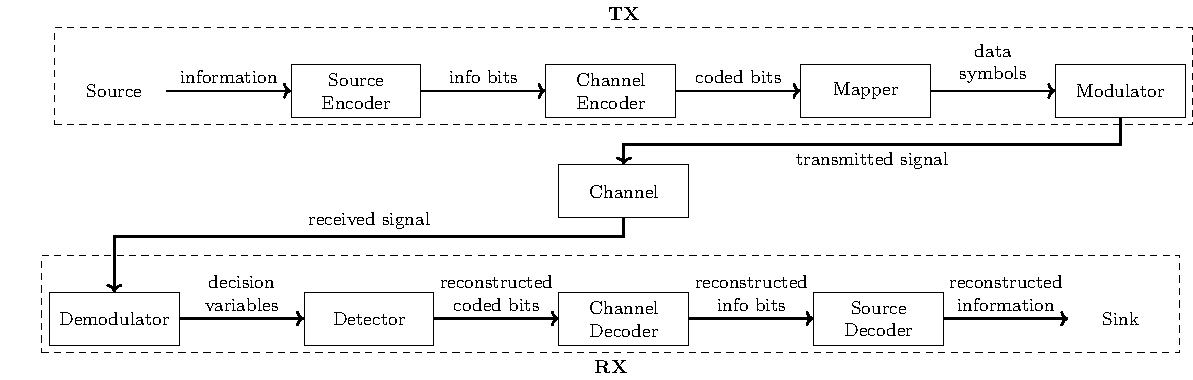
\includegraphics{figures/part1_background/out/digcom_system_block_diagram.pdf}}}
    \caption{Block diagram of a general digital communication system.}
    \label{fig:digcom_system_block_diagram}
\end{figure}

At the \ac{TX}, the information sequence is first processed by a source encoder to remove redundancy, followed by a channel encoder that introduces controlled redundancy to enable error detection.
The resulting coded bit sequence is partitioned into blocks of $m_c$ bits, each of which is mapped onto a complex-valued symbol drawn from a constellation $\mathcal{X}$ of size $2^{m_c}$.
The modulator then converts the symbol sequence into a baseband signal suitable for transmission.

During transmission, the channel distorts the signal due to attenuation, multipath propagation, and additive noise, such that the received signal differs from the transmitted signal.

At the \ac{RX}, the demodulator converts the received signal into a sequence of decision variables.
These are processed by the detector to obtain estimates of the originally transmitted symbols, which are then mapped back to coded bits.
Finally, the channel and source decoders reconstruct the original information sequence.

In this work, we consider a simplified version of this general architecture in order to focus on the aspects most relevant to our study.
Source coding and decoding are omitted, and the information is assumed to be available as a sequence of \ac{i.i.d.} bits without prior compression or digitization.
Channel coding and decoding are also not considered, such that the analysis is restricted to uncoded transmission.

The transmission medium is assumed to be a wireless channel affected by fading and additive noise. Furthermore, the channel is considered to be frequency-flat, meaning that its response remains constant over the entire signal bandwidth. The specific channel models used in this work are introduced in the relevant chapters.


\section{MIMO Communication Systems}

When both the \ac{TX} and the \ac{RX} are equipped with multiple antennas, the system is referred to as a \ac{MIMO} system.

Compared to a single-antenna link, the multiple antennas provide additional spatial degrees of freedom that can be exploited to increase data throughput, improve reliability, or achieve a trade-off between both.
Spatial multiplexing techniques enable significant capacity gains by transmitting multiple independent data streams simultaneously over different antennas. A well-known example is the BLAST architecture~\cite{foschini_1998}.
Alternatively, spatial diversity can be achieved through space-time coding schemes, which distribute symbols across both space and time to improve robustness against fading. A classical example is the Alamouti scheme~\cite{alamouti_1998}.
Throughout this work, the focus is on spatial multiplexing and, in particular, on how the simultaneous transmission of multiple data streams over a shared channel can be made most efficient through precoding.

\subsection{SU-MIMO}

In the point-to-point case, where a single \ac{TX} with $N_T$ antennas communicates with a single \ac{RX} with $N_R$ antennas, the system is called a \ac{SU} \ac{MIMO} system. A block diagram is shown in Fig.~\ref{fig:SU_MIMO_block_diagram_detailed}.

\begin{figure}[!ht]
    \centering
    \makebox[\textwidth][c]{\resizebox{1.2\textwidth}{!}{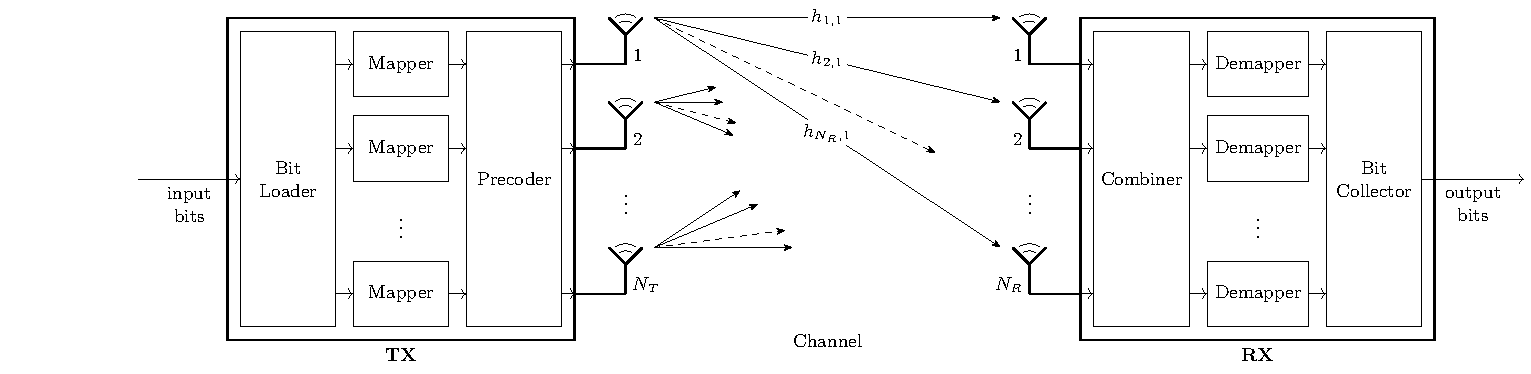
\includegraphics{figures/part1_background/out/su_mimo_block_diagram_detailed.pdf}}}
    \caption{Block diagram of a SU-MIMO system.}
    \label{fig:SU_MIMO_block_diagram_detailed}
\end{figure}

% channel input-output
The discrete-time complex baseband input-output relation of a \ac{SU}-\ac{MIMO} Gaussian channel is characterized by
\begin{equation}
    \mathbf{y} = \mathbf{H}\mathbf{x} + \mathbf{n},
\label{eq:su_mimo_io}
\end{equation}
where $\mathbf{x} \in \mathbb{C}^{N_T}$ is the transmitted signal vector, $\mathbf{y} \in \mathbb{C}^{N_R}$ is the received signal vector, $\mathbf{H} \in \mathbb{C}^{N_R \times N_T}$ is the channel matrix, and $\mathbf{n} \in \mathbb{C}^{N_R \times 1}$ is the additive noise vector.
The $(n_r, n_t)$-th entry of $\mathbf{H}$ represents the complex channel coefficient between transmit antenna $n_t$ and receive antenna $n_r$.
The noise vector is assumed to be circularly symmetric complex Gaussian, i.e., $\mathbf{n} \sim \mathcal{N}_{\mathbb{C}}(\mathbf{0}, N_0 \, \mathbf{I}_{N_R})$, such that its entries are spatially independent, each with an expected power of $N_0$.
The time index is omitted for brevity.

% transmitter
At the \ac{TX}, the information bits are divided into $N_S$ streams and mapped onto data symbols, which are collected in the vector $\mathbf{a} \in \mathbb{C}^{N_S \times 1}$.
Then, the transmitted signal is obtained by mapping the $N_S$ data symbol streams onto the $N_T$ transmit antennas according to a linear precoding scheme, represented by a matrix $\mathbf{F} \in \mathbb{C}^{N_T \times N_S}$.
The transmitted signal can therefore be expressed as
\begin{equation}
    \mathbf{x} = \mathbf{F} \, \mathbf{a}.
\label{eq:su_mimo_precoding}
\end{equation}
The data symbols are assumed to be zero-mean, mutually uncorrelated, and normalized, such that $ \mathbb{E}\!\left[\mathbf{a}\mathbf{a}^H\right] = \mathbf{I}_{N_S} $.
Throughout this work, the power allocation is assumed to be incorporated into the precoding matrix, unless explicitly stated otherwise. Under this convention, the total transmit power is constrained by
\begin{equation}
    \mathbb{E}\!\left[\|\mathbf{x}\|^2\right] = \mathrm{tr}\!\left(\mathbf{F}^H \mathbf{F}\right) \leq P_t.
\end{equation}
\begin{comment}
\begin{subequations}
\begin{align}
    P_t
    &\geq \mathbb{E}\!\left[ \left\|\mathbf{x}\right\|^2 \right] \\
    &= \mathbb{E}\!\left[ \mathbf{x}^H \mathbf{x} \right] \\
    &= \mathbb{E}\!\left[ \left(\mathbf{F} \mathbf{a}\right)^H \left(\mathbf{F} \mathbf{a}\right) \right] \\
    &= \mathbb{E}\!\left[ \mathbf{a}^H \mathbf{F}^H \mathbf{F} \mathbf{a} \right] \\
    &= \mathbb{E}\!\left[ \text{Tr}\!\left[ \mathbf{a}^H \mathbf{F}^H \mathbf{F} \mathbf{a} \right] \right] \\
    &= \mathbb{E}\!\left[ \text{Tr}\!\left[ \mathbf{F}^H \mathbf{F} \, \mathbf{a} \mathbf{a}^H \right] \right] \\
    &= \text{Tr}\!\left[ \mathbb{E}\!\left[ \mathbf{F}^H \mathbf{F} \, \mathbf{a} \mathbf{a}^H \right]  \right] \\
    &= \text{Tr}\!\left[ \mathbf{F}^H \mathbf{F} \, \mathbb{E}\!\left[ \mathbf{a} \mathbf{a}^H \right]  \right] \\
    &= \text{Tr}\!\left[ \mathbf{F}^H \mathbf{F} \, \mathbf{I}_{N_S} \right] \\
    &= \text{Tr}\!\left[ \mathbf{F}^H \mathbf{F} \right] \\
\label{eq:su_mimo_power_constraint_derivation}
\end{align}
\end{subequations}
\end{comment}

% receiver
At the \ac{RX}, the $N_R$ received signals are linearly combined to obtain the decision-variable vector $\mathbf{z} \in \mathbb{C}^{N_S \times 1}$.
The combiner is represented by a matrix $\mathbf{G} \in \mathbb{C}^{N_S \times N_R}$.
The decision variables can therefore be expressed as
\begin{equation}
    \mathbf{z} = \mathbf{G} \, \mathbf{y}.
\label{eq:su_mimo_combining}
\end{equation}
Based on $\mathbf{z}$, the detector forms estimates of the transmitted data symbols, which are then mapped back to bits.

% overall input-output
Substituting \eqref{eq:su_mimo_precoding} into \eqref{eq:su_mimo_io} and applying \eqref{eq:su_mimo_combining} yields the relation between the transmitted data symbols and the decision variables:
\begin{subequations}
\begin{align}
    \mathbf{z} &= \left(\mathbf{G} \, \mathbf{H} \, \mathbf{F}\right) \; \mathbf{a} + \mathbf{G} \, \mathbf{n}, \\
    &= \mathbf{T} \, \mathbf{a} + \mathbf{n_G},
\end{align}
\end{subequations}
where $\mathbf{T} \in \mathbb{C}^{N_S \times N_S}$ is the \ac{MIMO} transfer matrix and $\mathbf{n_G}$ represents spatially correlated Gaussian noise.
It is evident that, whenever the transfer matrix is not diagonal, the data symbols of different streams interfere with each other. The design of the precoding and combining matrices is therefore essential to suppress this inter-stream interference and improve overall system performance.

\subsection{MU-MIMO}

When multiple receivers are served simultaneously by a single multi-antenna transmitter, the system is referred to as a \ac{MU} \ac{MIMO} system. In this context, the transmitter is called the \ac{BS} and the individual receivers are referred to as \acp{UT}. A block diagram is shown in Fig.~\ref{fig:MU_MIMO_block_diagram}.

\begin{figure}[!ht]
    \centering
    \makebox[\textwidth][c]{\resizebox{0.8\textwidth}{!}{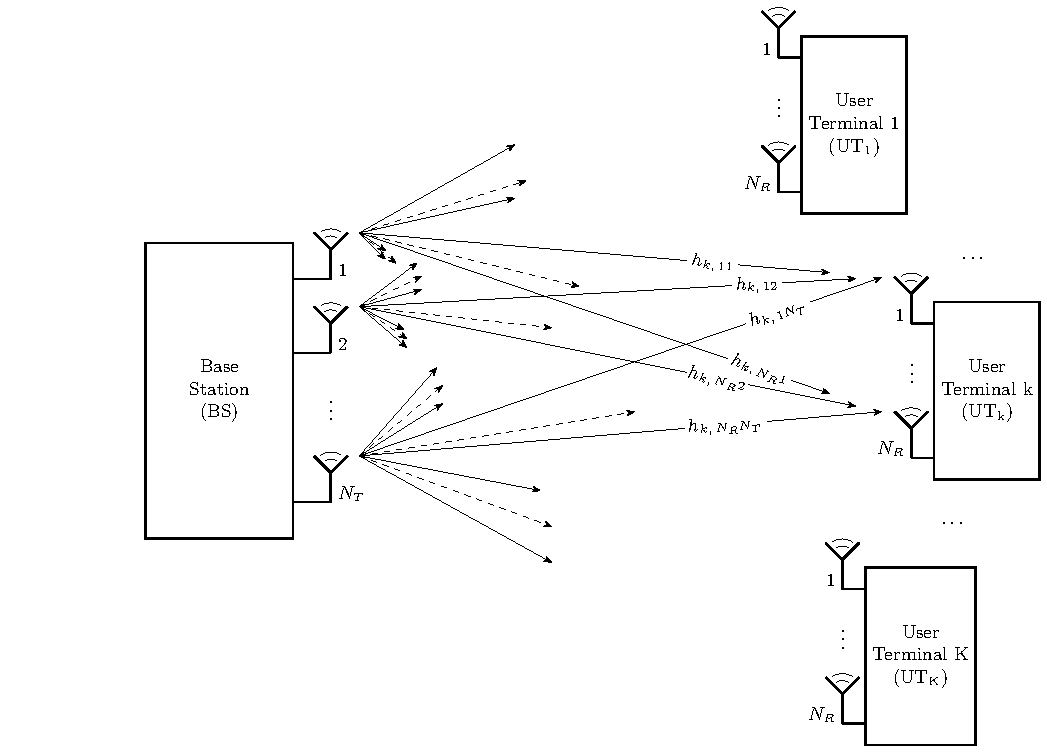
\includegraphics{figures/part1_background/out/mu_mimo_block_diagram.pdf}}}
    \caption{Block diagram of a MU-MIMO system.}
    \label{fig:MU_MIMO_block_diagram}
\end{figure}

% system dimension assumptions
Throughout this work, the \ac{BS} is assumed to be equipped with more antennas than all \acp{UT} combined, and each \ac{UT} is assumed to receive at most as many data streams as it has receive antennas.
For notational convenience, all \acp{UT} are assumed to receive the same number of data streams, denoted by $N_S$. In practical scenarios where this does not hold, $N_S$ is defined as the maximum number of data streams intended for any single \ac{UT}. The data symbol vectors intended for a \ac{UT} receiving fewer streams are padded with zeros.

% channel input-output
Analogous to the \ac{SU}-\ac{MIMO} case, the communication between the \ac{BS} and a certain \ac{UT}\textsubscript{k} is characterized by
\begin{equation}
    \mathbf{y}_k = \mathbf{H}_k \, \mathbf{x} + \mathbf{n}_k, \qquad k = 1, \dots, K,
\label{eq:mu_mimo_io}
\end{equation}
where $\mathbf{H}_k \in \mathbb{C}^{N_R \times N_T}$ is the channel matrix that describes the link between the \ac{BS} and \ac{UT}\textsubscript{k}.

% transmitter
The transmitted signal vector $\mathbf{x} \in \mathbb{C}^{N_T}$ is now a function of the data symbol vectors intended for different \acp{UT}. The \ac{BS} assigns a dedicated precoding scheme $\mathbf{F}_k \in \mathbb{C}^{N_T \times N_S}$ to the data symbol vector $\mathbf{a}_k$ intended for \ac{UT}\textsubscript{k}, and transmits the superposition of all precoded streams:
\begin{equation}
    \mathbf{x} = \sum_{k=1}^{K} \mathbf{F}_k \, \mathbf{a}_k.
\label{eq:mu_mimo_precoding}
\end{equation}
Since the data symbols intended for different \acp{UT} are considered to be uncorrelated, the total transmit power constraint can now be formulated as
\begin{equation}
    \mathbb{E}\!\left[\|\mathbf{x}\|^2\right] = \sum_{k=1}^{K} \mathrm{tr}\!\left(\mathbf{F}_k^H \mathbf{F}_k\right) \leq P_t.
\end{equation}
\begin{comment}
\begin{subequations}
\begin{align}
    P_t
    &\geq \mathbb{E}\!\left[ \left\|\mathbf{x}\right\|^2 \right] \\
    &= \mathbb{E}\!\left[ \mathbf{x}^H \mathbf{x} \right] \\
    &= \mathbb{E}\!\left[ \left(\sum_{k=1}^{K} \mathbf{F}_k \mathbf{a}_k\right)^H \left(\sum_{k'=1}^{K} \mathbf{F}_{k'} \mathbf{a}_{k'}\right) \right] \\
    &= \mathbb{E}\!\left[ \sum_{k=1}^{K} \left(\mathbf{F}_k \mathbf{a}_k\right)^H \left(\sum_{k'=1}^{K} \mathbf{F}_{k'} \mathbf{a}_{k'}\right) \right] \\
    &= \mathbb{E}\!\left[ \sum_{k=1}^{K} \sum_{k'=1}^{K} \left(\mathbf{F}_k \mathbf{a}_k \right)^H \mathbf{F}_{k'} \mathbf{a}_{k'} \right] \\
    &= \mathbb{E}\!\left[ \sum_{k=1}^{K} \sum_{k'=1}^{K} \mathbf{a}_k^H \mathbf{F}_k^H \mathbf{F}_{k'} \mathbf{a}_{k'} \right] \\
    &= \mathbb{E}\!\left[ \sum_{k=1}^{K} \sum_{k'=1}^{K} \text{Tr}\!\left[ \mathbf{a}_k^H \mathbf{F}_k^H \mathbf{F}_{k'} \mathbf{a}_{k'} \right] \right] \\
    &= \mathbb{E}\!\left[ \sum_{k=1}^{K} \sum_{k'=1}^{K} \text{Tr}\!\left[ \mathbf{F}_k^H \mathbf{F}_{k'} \, \mathbf{a}_{k'} \mathbf{a}_k^H \right] \right] \\
    &= \sum_{k=1}^{K} \sum_{k'=1}^{K} \text{Tr}\!\left[ \mathbf{F}_k^H \mathbf{F}_{k'} \, \mathbb{E}\!\left[ \mathbf{a}_{k'} \mathbf{a}_k^H \right] \right] \\
    &= \sum_{k=1}^{K} \sum_{k'=1}^{K} \text{Tr}\!\left[ \mathbf{F}_k^H \mathbf{F}_{k'} \, \mathbf{I}_{N_S} \, \delta_{kk'} \right] \\
    &= \sum_{k=1}^{K} \text{Tr}\!\left[ \mathbf{F}_k^H \mathbf{F}_{k} \right] \\
\end{align}
\end{subequations}
\end{comment}

% overall input-output
Applying the combining scheme $\mathbf{G}_k \in \mathbb{C}^{N_S \times N_R}$ at \ac{UT}\textsubscript{k} to the received signal vector and substituting \eqref{eq:mu_mimo_precoding} into \eqref{eq:mu_mimo_io} yields
\begin{equation}
    \mathbf{z}_k 
    = \underbrace{\left(\mathbf{G}_k \, \mathbf{H}_k \, \mathbf{F}_k\right) \; \mathbf{a}_k}_{\text{desired signal}}
    + \underbrace{\sum_{\substack{k'=1, \, k'\neq k}}^{K} \left(\mathbf{G}_k \mathbf{H}_k \mathbf{F}_{k'}\right) \, \mathbf{a}_{k'}}_{\text{inter-user interference}} 
    + \underbrace{\mathbf{G}_k \, \mathbf{n}_k}_{\text{noise}}.
    \label{eq:mu_mimo_effective}
\end{equation}
The key difference from the \ac{SU}-\ac{MIMO} scenario is the presence of inter-user interference. Each \ac{UT} receives not only its desired signal but also the signals intended for all other \acp{UT}. Suppressing this interference through precoder design at the \ac{BS} is an important challenge in \ac{MU}-\ac{MIMO} systems.

% compact notation
The overall input-output relation of the \ac{MU}-\ac{MIMO} Gaussian channel can be written compactly as
\begin{gather}
    \mathbf{z} = \left(\mathbf{G} \, \mathbf{H} \, \mathbf{F}\right) \; \mathbf{a} + \mathbf{G} \, \mathbf{n}, \quad \text{with} \\
    \quad \mathbf{z} = \begin{bmatrix} \mathbf{z}_1 \\ \vdots \\ \mathbf{z}_K \end{bmatrix},
    \quad \mathbf{G} = \begin{bmatrix} \mathbf{G}_1 & & \\ & \ddots & \\ & & \mathbf{G}_K \end{bmatrix},
    \quad \mathbf{H} = \begin{bmatrix} \mathbf{H}_1 \\ \vdots \\ \mathbf{H}_K \end{bmatrix}, 
    \quad \mathbf{F} = \begin{bmatrix} \mathbf{F}_1 & \dots & \mathbf{F}_K \end{bmatrix}, 
    \quad \mathbf{a} = \begin{bmatrix} \mathbf{a}_1 \\ \vdots \\ \mathbf{a}_K \end{bmatrix}. \notag
\end{gather}
where $\mathbf{G} \in \mathbb{C}^{K N_S \times K N_R}$ denotes the compound combining matrix, $\mathbf{H} \in \mathbb{C}^{K N_R \times N_T}$ the compound channel matrix, and $\mathbf{F} \in \mathbb{C}^{N_T \times K N_S}$ the compound precoding matrix.


\section{Mutual Information and Capacity}


